\section{Introduction}

Many of our concepts and words are vague. A vague category knows clear
cases that fall under it, clear cases that do not, and also so-called
borderline cases. Borderline cases neither clearly apply, nor clearly
not apply, and there may be differences between borderline cases in
terms of how well they represent the category in question. Vagueness
does not seem to dramatically affect the success of everyday
communication, but it is troublesome for some of our theories of
language. This is especially the case for the logico-semantic
tradition of Frege, Russell and the young Wittgenstein which is
challenged by the paradoxes vagueness gives rise to. As can be
expected, many proponents of this tradition have tried to address the
problem, ranging from suggesting that there is nothing wrong with the
classical approach since the problem is of a different nature, as in
Williamson's epistemic view~\citep*{Williamson1994:Vagueness}, to
proposing various kinds of modifications to either semantics, logic,
or both, as in for example supervaluationism
\citep[e.g.][]{Mehlberg1958,Fine1975}, many-valued logic
\citep[e.g.][]{Zadeh1975,Machina1976,Edgington1997}, or paraconsistent
logic \citep[e.g.][]{CobrerosEgre2012:Tolerant-Classi}.

Yet there are other intriguing aspects about vagueness. The
puzzle that we are concerned with here is how vagueness could arise
and be maintained in the first place. This may not seem a particularly
deep issue at first glance, but on closer inspection it is a serious
worry to functionalist accounts that maintain that our concepts and
language use evolved in order to be efficient. Since the existence of
unclear borderline cases seems to entail inefficiency of
categorization or communication, the challenge, succinctly put forward
by \citet{Lipman2009:Why-is-Language}, is to explain how vagueness can
exist despite its obvious and demonstrable functional deficiency under
evolutionary pressure to be optimally expressive.

This problem, call it Lipman's problem, has a conceptual and a
technical side to it. Conceptually, it asks for reasons and general
mechanisms by which we could plausibly conceive of vagueness as
resisting the pressure of evolutionary selection for precision. Such
reasons and general mechanisms are, arguably, not hard to imagine.
But each putative explanation, no matter how plausible intuitively,
must also be checked for internal consistency and its potential to
account for the fact that we see vagueness as a part of a by-and-large
efficient system of categorization and communication. In other words,
not all first-shot rebuttals of Lipman's problem will do. Denying that
there is any functional pressure on efficient communication, for
instance, is a non-starter, because it leaves the relative efficiency
of our communication with vague words entirely unexplained. In sum,
the technical answer to Lipman's problem is to give, ideally, a
conceptually sound model of evolution of categorization or language
use that yields by-and-large efficient categories \emph{and}
vagueness.

A number of authors have recently tried to explain why vagueness
evolved, based on considerations why a vague language might be useful
\citep[e.g.][]{Jaegherde-Jaegher2003:A-Game-Theoreti,Deemter2009:Utility-and-Lan,Jaegherde-JaegherRooijvan-Rooij2010:Strategic-Vague,BlumeBoard2013:Intentional-Vag}. In
contrast to these, others have argued that vagueness is a natural
byproduct of limitations in information processing
\citep[e.g.][]{FrankeJager2010:Vagueness-Signa,OConnor2013:The-Evolution-o}. This
paper makes a contribution to the latter line of thought.  Concretely,
we introduce the replicator diffusion dynamics ---a novel variant of
the replicator mutator dynamic--- that integrates stochastic noise on
the differential confusability of similar stimuli. Our main
contribution, therefore, is a technical answer to Lipman's problem in
the sense introduced above. The dynamic proposed here generalizes and
complements previous like-minded accounts. We show that stochastic
noise can not only lead to vague, yet communicative efficient signal
use, but can also unify evolutionary outcomes and help avoid
suboptimal categorization.

The next section introduces the background against which the work
presented here can be appreciated. Section~\ref{sec:repl-diff-dynam}
introduces the replicator diffusion dynamic and elaborates on its
relation with the replicator mutator
dynamic. Section~\ref{sec:exploring-rdd} explores the replicator
diffusion dynamic on the relevant class of generalized signaling games
introduced in
Section~\ref{sec:background}. Section~\ref{sec:discussion} reflects on
the results and compares what has been achieved to related accounts in
more detail. 

\section{Background}
\label{sec:background}

The view that vagueness is a natural concomitant of cognitive
limitations of language users has been formalized in a number of ways,
using evolutionary game theory and certain generalizations of
signaling games, so called \emph{similarity-maximizing games}, or
\emph{sim-max games}, for short
\citep{FrankeJager2010:Vagueness-Signa,OConnor2013:Evolving-Percep,OConnor2013:The-Evolution-o}. Our
contribution is best seen in relation to these accounts, as it also
relies on sim-max games. Let's introduce these first, and then zoom in
on the problem of vagueness.

\subsection{Sim-max games \& conceptual spaces}

Signaling games, as introduced by \citet{Lewis_1969:Convention}, have
a sender and a receiver. The sender knows the true state of the world,
but the receiver does not. The sender can select a signal, or message,
to reveal to the receiver, who then chooses an act. In Lewis' games,
states are maximally distinct from each other and the receiver's acts
are related to them one-to-one. If the receiver chooses the act that
corresponds to the actual state, the play is a success, otherwise a
failure. Certain regular combinations of sender signaling and receiver
reaction make messages meaningful, in the sense that their use is
correlated systematically to certain states or acts. To investigate
the conditions under which such meaning-generating behavior can evolve
is a highly interesting topic that we are only beginning to fully
understand
\citep[e.g.][]{Warneryd1993:Cheap-Talk-Coor,BlumeKim1993:Evolutionary-St,Zollman2005:Talking-to-Neig,Huttegger2007:Evolution-and-t,Pawlowitsch2008:Why-Evolution-d,Barrett2009:The-Evolution-o,Wagner2009:Communication-a,HutteggerSkyrms2010:Evolutionary-Dy,Skyrms2010:Signals,HutteggerZollman2011:Signaling-Games}.

Similarity-maximizing games are generalizations of Lewis' games in
that they allow different states to be more or less similar to one
another, and, roughly put, make success of communication a function of
that similarity. Intuitively speaking, while Lewis' games treated
communicative success as a matter of black and white, sim-max games
allow for a gradient notion of communicative success: the more similar
the receiver's interpretation is to the actual state, the more
successful the play is taken to be. Signaling games with
utility-relevant similarities in the state space are fairly standard
in economics
\citep[e.g.][]{Spence1973:Job-market-sign,CrawfordSobel1982:Strategic-Infor},
but have received particular attention in a more philosophical and
linguistic context for reasons that will become clear presently
\citep{Jager2007:The-Evolution-o,JagerRooijvan-Rooij2007:Language-Struct,JagerMetzger2011:Voronoi-Languag}.

A sim-max game, in the relevant sense here, consists of a set of
states $\States$, a set of messages $\Messgs$ with much fever messages
than states, a prior probability distribution $\Pr \in
\Delta(\States)$ that gives the occurrence probabilities of states, a
similarity metric on states $\similarity \mycolon \States \times
\States \rightarrow \mathds{R}$, and a utility function $\Utils
\mycolon \States \times \States \rightarrow \mathds{R}$. We identify
the receiver's acts with the states of the world, so that the game is
one of guessing the actual state, so to speak. We also assume that
sender's and receiver's interests are alike, so we only have one
utility function. We do not consider message costs, so utilities only
depend on the actual state, and the receiver's response. The
similarity function should satisfy the usual requirements for a
metric:
\begin{align*}
  & \similarity(\mystate{1}, \mystate{2}) \ge 0 &&
  \similarity(\mystate{1}, \mystate{2}) = 0 \Leftrightarrow
  \mystate{1} = \mystate{2} \\
  & \similarity(\mystate{1}, \mystate{2}) = \similarity(\mystate{2},
  \mystate{1}) && \similarity(\mystate{1}, \mystate{2}) \le
  \similarity(\mystate{1}, \mystate{3}) + \similarity(\mystate{3}, \mystate{2})\,.
\end{align*}
The utility function should be a monotonically decreasing function of
similarity:
\begin{align*}
  \similarity(\mystate{1},\mystate{2}) \ge
  \similarity(\mystate{1},\mystate{3}) \ \ \Rightarrow \ \ 
  \Utils(\mystate{1},\mystate{2}) \ge
  \Utils(\mystate{1},\mystate{3})\,.
\end{align*}
To keep matters simple, we here only look at cases where $\States$
contains finitely many points from the unit interval, all of which
have equal probability, and with similarity given by the Euclidean
distance in this one-dimensional space.

\citet{JagerMetzger2011:Voronoi-Languag} showed that the
evolutionarily stable states of sim-max games are remarkably
systematic. Their results were obtained for games with infinitely many
states in $n$-dimensional Euclidean space $\States \subseteq
\mathds{R}^n$ and a quadratic loss function for utilities
$\Utils(\mystate{1}, \mystate{2}) = - (\mystate{1} -
\mystate{2})^2$. For these games, the evolutionarily stable states are
demonstrably so-called Voronoi-languages. Intuitively speaking, a
Voronoi language is a pair of sender and receiver strategies, such
that the sender strategy (quasi-)partitions the state space into
convex categories, while the receiver's interpretations are the
central spots in each category. Figure~\ref{fig:VoronoiLanguage} gives
an example of such a Voronoi-language for a sim-max game with $\States
= [0,1]$, two messages, and a flat prior distribution over states. The
sender uses one message exclusively for all points in the lower half
of the interval and another for all points in the upper half. The
receiver's interpretations of messages are the central points in the
respective intervals.

\begin{figure}
  \centering

  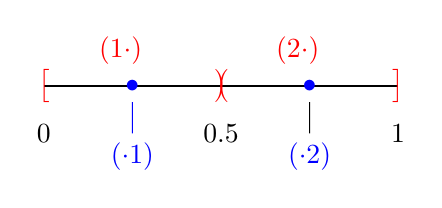
\begin{tikzpicture}[scale=3]

        \begin{scope}

          \draw[-,thick] (0,0) -- (1.5,0);

          \draw (0,0) node {\color{red}{\big{[}}};

          \draw (.75,0) node {\color{red}{\big{)}}};

          \draw (.76,0) node {\color{red}{\big{(}}};

          \draw (1.5,0) node {\color{red}{\big{]}}};

            \draw (.325,.15) node
            {\color{red}{$\Spure(\mymessg{1}  \probbar \cdot)$}};

            \draw (1.075,.15) node
            {\color{red}{$\Spure(\mymessg{2} \probbar \cdot)$}};

            \node at (.375,0) (node1) {\color{blue}{$\bullet$}};

            \node at (.375,-.3) (label1)
            {\color{blue}{${\Rpure}(\cdot \probbar \mymessg{1})$}};

            \draw[-,color=blue] (node1) -- (label1);

            \node at (1.125,0) (node2) {\color{blue}{$\bullet$}};

            \node at (1.125,-.3) (label2)
            {\color{blue}{${\Rpure}(\cdot \probbar \mymessg{2})$}};

            \draw[-] (node2) -- (label2);

            \draw (0,-.2) node {$0$};

            \draw (.75,-.2) node {$0.5$};

            \draw (1.5,-.2) node {$1$};

          \end{scope}
 
        \end{tikzpicture}

        \caption{Example of a Voronoi-language on $\States =
          [0,1]$. The (pure) sender strategy $\Spure \in
          \Messgs^\States$ uses one signal for the lower half, and
          another for the upper half of the unit interval. The (pure)
          receiver strategy $\Rpure \in \States^\Messgs$ selects the
          central elements in the respective intervals.}
  \label{fig:VoronoiLanguage}
\end{figure}


This result is interesting, because it demonstrates that signaling can
impose orderly categories on a metric space, without that being the
ulterior purpose of it all. Sender and receiver can be distinct
entities, whose purpose is to communicate effectively about the actual
state. In that case, evolving Voronoi-languages would explain why
linguistic categories are well-behaved and orderly in the way they
appear to be. More abstractly, sender and receiver can also be thought
of as distinct modules in a single system, where the first module must
discretize the information by selecting a small sample of,
suggestively, category labels. These are passed to a second module
that tries to decode the original information. In this case, evolving
Voronoi-languages would explain why conceptual categories are
well-behaved and orderly in the way that they appear to be
\citep[e.g.][for more on this latter
interpretation]{OConnor2013:Evolving-Percep}.

Seen in this light, sim-max games appear to have the potential of
providing a foundation to approaches in cognitive semantics that rely
on the notion of conceptual spaces.
\citet[][70--77]{Gardenfors2000:Conceptual-Spac}, for example, has
prominently argued that natural categories are convex regions in
conceptual space. If the conceptual space has a suitable metric, then
it is possible to think of these convex categories as derived from a
set of prototypes. Fixing a set of prototypes, we consider the
category corresponding to each prototype $p$ as the set of points that
are more similar to $p$ than to any other
\citep[e.g.][]{OkabeBoots2000:Spatial-Tessell}. In this way,
\citet{Gardenfors2000:Conceptual-Spac} argues, an efficient
categorization system can be obtained: storing the prototypes lets us
recover the categories without having to store each category's
extension. However, what is left unexplained so far, is where the
prototypes come from, and why we would not see just any distribution
of prototypes as an equally efficient classification system. This is
where sim-max games can contribute a principled approach to deriving,
in an independent way, not only convex categories but also
prototypical exemplars belonging to them.


\subsection{Vague signaling in sim-max games}

This brief outline of an approach to conceptual categorization using
sim-max games leaves many problems unaddressed. One of them is that
natural categories for continuously variable stimuli, like shades of
color, pitch heights, spatial dimension and the like, do not have
unique, point-valued prototypes and clear category boundaries. We
would like to account for the possibility of such vagueness, and that
means in particular for the following criteria
\citep[e.g.][]{Sainsbury1991:Is-There-Higher,KeefeSmith1997:Vagueness:-A-Re,Smith2008:Vagueness-and-D}:
(i) clear positive examples of a vague category should show a
gradient, perhaps smooth, transition to clear negative examples to
accommodate also higher-order vagueness; (ii) prototypes should
likewise be gradient regions, peaking at the center of the vague
category they represent.


\citet{DouvenDecock2011:Vagueness:-A-Co} show that
\citeauthor{Gardenfors2000:Conceptual-Spac}'s conceptual spaces
approach can be extended to account for the existence of borderline
cases. From the assumption that prototypes are not unitary points, but
extended, yet convex regions in conceptual space,
\citeauthor{DouvenDecock2011:Vagueness:-A-Co} give a construction
algorithm that yields ``collated Voronoi diagrams'' with thick,
extended boundaries representing borderline regions. Building on this
work, \citet{DecockDouven2012:What-is-Graded-} show further how it is
possible to arrive at higher-order vagueness and degrees of category
membership, by, essentially, weighing in the distance of different
borderline cases to various prototypical regions. This accounts for
the first of the two desiderata mentioned above, but still assumes
that crisp non-gradient prototype regions must be pre-given.

An alternative approach is taken by
\citet{FrankeJager2010:Vagueness-Signa} and
\citet{OConnor2013:The-Evolution-o} who show how the above desiderata
can be met by evolving strategies in sim-max games for various types
of solution concepts. These can be divided into micro- and macro-level
approaches. Micro-level approaches look at adaptive behavior of
individual agents. Usually, changes in the behavioral dispositions of
agents occur after every single interaction. In contrast, macro-level
approaches outline more abstract, aggregate dynamics, happening in a
population of agents, or otherwise abstracting from seemingly
irrelevant detail. Usually, a macro-level dynamic captures changes of
frequencies of behavioral types in the population over time.

As for micro-dynamics, \citet{FrankeJager2010:Vagueness-Signa} show
how limited memory of past interactions can lead to vague signal use,
when averaging over a single agent's behavior over time or over the
momentary behavior of a population of several language
users. \citet{OConnor2013:The-Evolution-o} introduces a variant of
reinforcement learning that entails a low-level form of stimulus
generalization. Agents update their behavior after each round of play
in such a way that states similar to the one that actually occurred
are subject to behavioral adjustment as well. (A more detailed
discussion of alternative approaches is deferred until
Section~\ref{sec:discussion}, where we can compare them better with the
system introduced in this paper.)

\citet{FrankeJager2010:Vagueness-Signa} also consider a macro-level
approach, using the notion of a \emph{quantal response}. A quantal
response function is a probabilistic choice rule that formalizes the
idea that agents make small mistakes when calculating the expected
utility of choice options. In aggregation, these probabilistic
mistakes lead to systematic ``trembles'' that produce vague signal
use. The approach we take here is superficially similar, but there are
crucial differences. For one, we adopt a dynamic perspective by
looking at limited-time outcomes of a dynamic process. For another, we
demonstrate in Section~\ref{sec:discussion} that quantal responses can
give rise to counterintuitive predictions. These counterintuitive
examples suggest that vagueness in sim-max games is not convincingly
explained by appeal to mistakes in calculating expected utility, but
rather, as we assume here, as the result of confusing similar
states.




%%% Local Variables: 
%%% mode: latex
%%% TeX-master: "paper"
%%% TeX-PDF-mode: t
%%% End:



